\documentclass[a4paper, 11pt]{article}


\usepackage[slovak]{babel}
\usepackage[utf8]{inputenc}
\usepackage[left=2cm, top=3cm, text={17cm, 24cm}]{geometry}
\usepackage{times}
\usepackage{verbatim}
\usepackage{enumitem}
\usepackage{graphicx}
\usepackage{listings}
\usepackage{color}
\usepackage[unicode]{hyperref}
\usepackage{tabularx}
\usepackage{parskip}
\usepackage[slovak, boxed]{algorithm2e}
\hypersetup{
    colorlinks=true,
    linkcolor=black,
    urlcolor=blue, 
    citecolor=blue
}
\definecolor{mygreen}{rgb}{0,0.6,0}
\definecolor{mygray}{rgb}{0.5,0.5,0.5}
\definecolor{mymauve}{rgb}{0.58,0,0.82}
\lstset{
  backgroundcolor=\color{white},
  basicstyle=\footnotesize,
  breaklines=true,
  captionpos=b,
  commentstyle=\color{mygreen},
  escapeinside={\%*}{*)},
  keywordstyle=\color{blue},
  stringstyle=\color{mymauve},
  tabsize=4
}
\setlength{\parindent}{0pt}
\setlength{\parskip}{1em}

\begin{document}

	%%%%% Titulná stránka %%%%%
	\begin{titlepage}
		\begin{center}
			
\includegraphics[width=0.77\linewidth]{res/logo_FIT.pdf} \\

			\vspace{\stretch{0.382}}

			\Huge{IMAP klient s podporou TLS} \\
			\LARGE{Manuál} \\
			\Large{Autor: Adam Ližičiar (xlizic00)}
			\vspace{\stretch{0.618}}
		\end{center}

		\begin{minipage}{0.4 \textwidth}
			{\Large \today}
		\end{minipage}
		\hfill
	\end{titlepage}



	%%%%% Obsah %%%%%
	\pagenumbering{roman}
	\setcounter{page}{1}
	\tableofcontents
	\clearpage



	%%%%% Introduction %%%%%
	\pagenumbering{arabic}
	\setcounter{page}{1}


	\section{Úvod}
	Hlavným zmyslom tohto programu je umožniť používateľovi čítanie emailov zo svojej emailovej schránky pomocou IMAP(S) protokolu s možnou podporou šifrovacieho protokolu TLS.\newline

	%%%%% Implementace %%%%%
	\section{Hlbšia analýza problematiky}
	IMAP (Internet Message Access Protocol)\cite{rfc3501} je protokol, ktorý sa používa na vzdialený prístup k e-mailovým správam uloženým na serveri. Je to jeden z najpoužívanejších protokolov na čítanie e-mailov a bol vyvinutý s cieľom poskytnúť synchronizovaný prístup k e-mailovým schránkam. Na rozdiel od POP3 (Post Office Protocol 3), ktorý sťahuje správy do počítača a maže ich zo servera, IMAP umožňuje užívateľom spravovať správy na serveri bez ich sťahovania, čím sa zabezpečuje prístup k e-mailu z viacerých zariadení. \newline
	IMAP protokol vykonáva textové príkazy cez sériu príkazov, v ktorej klient posiela požiadavku serveru, napríklad na získanie zoznamu správ alebo stiahnutie konkrétnej správy. Server následne odpovie s požadovanými informáciami. Tento protokol má tiež funkcie, ako je označovanie správ (napr. neprečítané, vymazané), filtrovanie a vyhľadávanie správ na serveri.\newline
	IMAPS (IMAP over SSL/TLS) je verzia IMAP protokolu, ktorá zahŕňa šifrovanie komunikácie medzi klientom a serverom prostredníctvom protokolu TLS (Transport Layer Security). TLS\cite{rfc5246} je šifrovací protokol, ktorý zabezpečuje bezpečnú komunikáciu. Cieľom TLS je zabezpečiť, aby údaje odosielané medzi dvoma zariadeniami neboli odpočúvané, zneužité alebo zmenené.\newline
	Pri použití IMAPS sa najprv nadviaže obyčajné (nešifrované) spojenie, a až potom sa nastavia bezpečnostné parametre na šifrovanie prenosu údajov. \newline
	IMAP(S) protokol využíva sériu príkazov, ktoré klient posiela serveru na vykonanie rôznych operácií s e-mailovými správami. Medzi základné príkazy patria: \texttt{SELECT} na výber konkrétnej poštovej schránky, \texttt{EXAMINE} na získanie informácií o poštovej schránke bez jej výberu, \texttt{FETCH} na stiahnutie konkrétnej správy alebo časti správy, \texttt{STORE} na zmenu atribútov správy (napríklad označenie ako prečítané alebo odstránené), \texttt{SEARCH} na vyhľadávanie správ podľa určitých kritérií, \texttt{LIST} a \texttt{LSUB} na získanie zoznamu poštových schránok, a \texttt{LOGOUT} na ukončenie spojenia. 


	\section{Používanie programu}
	Program sa spúšťa s nasledujúcimi parametrami:
	\begin{lstlisting}
	./imapcl server [-p port] [-T [-c certfile] [-C certaddr]]
	[-n] [-h] -a auth_file [-b MAILBOX] -o out_dir
	\end{lstlisting}		
	Poradie parametrov je ľubovoľné. Popis parametrov je nasledovný:
	\begin{itemize}
		\item Povinný je názov servera (IP adresa alebo doménové meno) požadovaného zdroja.
		\item Voliteľný parameter \texttt{-p port} špecifikuje číslo portu na serveri. 
		\item Parameter \texttt{-T} zapína šifrovanie (\texttt{imaps}), ak nie je uvedený, použije sa nešifrovaná verzia protokolu.
		\item Voliteľný parameter \texttt{-c} označuje súbor s certifikátmi, ktorý sa použije na overenie platnosti certifikátu SSL/TLS predloženého serverom.
		\item Voliteľný parameter \texttt{-C} určuje adresár, v ktorom sa majú vyhľadávať certifikáty na overenie platnosti certifikátu SSL/TLS predloženého serverom. Výchozia hodnota je \texttt{/etc/ssl/certs}.
		\item Pri použití parametra \texttt{-n} sa bude pracovať iba s novými správami.
		\item Pri použití parametra \texttt{-h} sa budú sťahovať iba hlavičky správ.
		\item Povinný parameter \texttt{-a auth\_file} odkazuje na súbor s autentifikačnými údajmi.
		\item Parameter \texttt{-b} špecifikuje názov schránky, s ktorou sa bude na serveri pracovať. Výchozia hodnota je \texttt{INBOX}.
		\item Povinný parameter \texttt{-o out\_dir} určuje výstupný adresár, do ktorého má program uložiť stiahnuté správy.
	\end{itemize}

	\section{Architektúra programu}
	Program je navrhnutý ako modulárny systém s využitím objektovo-orientovaného prístupu. Architektúra zahŕňa viacero tried, z ktorých má každá jasne definovanú úlohu, čím je zabezpečená prehľadnosť a jednoduchá rozšíriteľnosť. Hlavné riadenie programu je implementované prostredníctvom konečného stavového automatu (viď. \ref{subsection:usecase}), ktorý spravuje prechod medzi stavmi, ako sú autentifikácia, výber schránky či sťahovanie správ.\newline
	Komunikácia medzi klientom a serverom prebieha podľa protokolu IMAP(S).\newline
	Pre zabezpečenie stability programu je implementovaný systém spracovania chýb. Využíva sa mechanizmus výnimiek, ktorý identifikuje rôzne druhy chýb s vlastnými  chybovými kódmi.\newline
	Pri vytváraní niektorých komentárov v kódoch a pri doplnení niektorých testov bol použitý nástroj Gemini od firmy Google kvôli zahrnutiu čo najväčšieho spektra rôznych testov, ktorým je program podrobený. Tento nástroj bol použitý výlučne iba na tieto dve veci a nie na tvorbu architektúry alebo funkcií v programe.

	\subsection{Hlavné riadenie programu}
	Hlavné riadenie programu prebieha pomocou diagramu prípadov použitia, ktorý je implementovaný v súboroch \texttt{src/classes/FiniteStateMachine/FiniteStateMachine.\{cpp, hpp\}}. Samotné ovládanie pomocou tohto diagramu je implementované v súbore \texttt{src/classes/IMAPClient.cpp} vďaka \texttt{while} cyklu. Vo \texttt{while} cykle sú použité podmienky \texttt{if-else} namiesto \texttt{switch}-u kvôli lepšej prehľadnosti kódu.\newline
	Daný diagram je možné vidieť v prílohe \ref{subsection:usecase}.
	\begin{algorithm}[ht]
		\SetKw{Break}{break}
		
		\While{FSM.getState() $\neq$ END}{
			\uIf{FSM.getState() == INIT}{
				FSM.transitionToAuth()\;
			}
			\uElseIf{FSM.getState() == AUTH}{
				\If{loginSuccessful()}{
					FSM.transitionToSelect()\;
				} \Else {
					FSM.transitionToEnd()\;
				}
			}
			\uElseIf{FSM.getState() == SELECT}{
				\If{mailboxExists()}{
					FSM.transitionToDownload()\;
				} \Else {
					FSM.transitionToQuit()\;
				}
			}
			\uElseIf{FSM.getState() == DOWNLOAD}{
				downloadEmails()\;
				FSM.transitionToQuit()\;
			}
			\uElseIf{FSM.getState() == QUIT}{
				logout()\;
				FSM.transitionToEnd()\;
			}
			\Else{
				throwError()\;
			}
		}
		\caption{Zjednodušený pseudokód FSM cyklu implementovaného v triede \texttt{IMAPClient}.}
		\label{algorithm:fsm_loop_simple}
		\end{algorithm}

	\subsection{Triedy a ich funkcionalita}
	Grafické zobrazenie diagramu tried je možné vidieť v prílohe \ref{subsection:class}. Program sa skladá zo siedmych tried, ktoré majú nasledujúcu funkcionalitu:
	\begin{itemize}
		\item \textbf{FiniteStateMachine} \\
		Trieda riadi tok programu pomocou konečného stavového automatu (FSM). Obsahuje stavy programu a metódy na ich prechod, a to konkrétne stavy INIT, AUTH, SELECT, DOWNLOAD, QUIT a END (viď \ref{subsection:usecase}).
	
		\item \textbf{AuthManager} \\
		Spravuje autentifikáciu používateľa. Zabezpečuje získanie prihlasovacích údajov a ich správne uloženie do tejto triedy. Autentifikačný súbor musí mať formát \texttt{username =  xxx} a na ďalšom riadku \texttt{password =  yyy}. Pri neexistujúcom súbore skončí program vyvolaním výnimku a pri nesprávnych údajoch skončí program s nulovým návratovým kódom a oznámením, že sa nepodarilo overiť identitu na strane servera.
	
		\item \textbf{ArgsParser} \\
		Zodpovedá za spracovanie argumentov príkazového riadku. Umožňuje používateľovi zadať konfiguráciu, ako je názov servera, portu, a ďalšie možnosti.
	
		\item \textbf{Message} \\
		Reprezentuje e-mailovú správu. Obsahuje údaje ako odosielateľ, predmet, telo správy a prílohy, pričom umožňuje manipuláciu s týmito údajmi. Táto trieda obsahuje funkciu \texttt{decodeMime()}, ktorej tvorba bola inšpirovaná funkciami z knižnice \texttt{mimetic}. Funkcia dokáže zmeniť niektoré druhy MIME textov, aby boli prehľadné pre používateľa tohto programu.
	
		\item \textbf{MessageFactory} \\
		Zodpovedá za vytváranie inštancií správ. Prijíma surové dáta zo servera a transformuje ich na objekt typu `Message`. Po spracovaní týchto dát je každá e-mailová správa uložená do vlastného súboru, ktorý má nazov vo formáte \texttt{SUBJECT\_IDMESSAGE.txt}. Tento názov bol zvolený pretože je jedinečný pre akékoľvek emailové správy (vďaka IDMESSAGE) a zároveň je prehľadný kvôli použitiu predmetu správy v názve. V tejto triede taktiež prebieha obsluha lokálneho súboru, ktorý obsahuje potrebné údaje pre správnu synchronizáciu dát. Po stiahnutí prvých správ vznikne v priečinku s emailami pod názvom \texttt{imapcl.log}.
	
		\item \textbf{IMAPConnection} \\
		Spravuje spojenie so serverom pomocou protokolu IMAP(S). Umožňuje odosielať príkazy na server, prijímať odpovede a spracúvať komunikáciu\cite{opennsslapi}. V tejto triede je vo funckii na prijatie odpovedí zabudovaný časovač, ktorý má dĺžku 10 sekúnd a slúži na ukončenie programu v prípade, že by server prestal odpovedať.
	
		\item \textbf{IMAPClient} \\
		Hlavná trieda, ktorá integruje všetky ostatné komponenty. Implementuje logiku programu na riadenie stavového automatu, vykonáva autentifikáciu a sťahovanie e-mailových správ.
	\end{itemize}	

	\subsection{Komunikácia klienta so serverom}
	V rámci implementácie triedy \texttt{IMAPClient} prebieha komunikácia klienta so serverom v jednotlivých krokoch (viď. sekvenčný diagram v prílohe \ref{subsection:sequence}), ktoré zodpovedajú stavovému diagramu FSM (viď \ref{subsection:usecase}). Medzi kroky použité v tomto programe komunikácie patria:

	\begin{itemize}
		\item \textbf{Prihlásenie (LOGIN)} \\
		Klient odošle príkaz \texttt{LOGIN} s prihlasovacími údajmi (meno používateľa a heslo). Server následne odpovie, či bola autentifikácia úspešná (\texttt{OK}), alebo zlyhala.

		\item \textbf{Výber schránky (SELECT)} \\
		Klient odošle príkaz \texttt{SELECT} s názvom e-mailovej schránky, z ktorej chce používateľ čítať e-mailovú poštu. Server odpovie, či je schránka dostupná. V prípade sťahovania neprečítaných správ je použitý príkaz \texttt{UNSEEN}, pretože stiahnutie ešte nepredpokladá, že danú správu používateľ aj naozaj prečíta, a preto ju nechá označenú ako neprečítanú.

		\item \textbf{Vyhľadávanie správ (SEARCH)} \\
		Klient pomocou príkazu \texttt{SEARCH} vyhľadá správy podľa zadaných kritérií (napr. neprečítané správy, všetky správy). Server odpovie zoznamom UID správ, ktoré vyhovujú podmienkam.

		\item \textbf{Sťahovanie správ (FETCH)} \\
		Po získaní UID správ klient odošle príkaz \texttt{FETCH}, aby stiahol obsah správ. Požaduje buď len hlavičky (\texttt{BODY.PEEK[HEADER]}) alebo celé telo správ (\texttt{BODY[]}). Stiahnuté správy sa spracujú a následne lokálne uložia.

		\item \textbf{Odhlásenie (LOGOUT)} \\
		Po ukončení práce klient odošle príkaz \texttt{LOGOUT}, čím uzavrie spojenie so serverom. Server odpovie potvrdením ukončenia komunikácie.
	\end{itemize}
	Každý krok komunikácie je realizovaný prostredníctvom odoslania príkazov serveru a spracovania odpovedí. Tieto kroky zaisťujú správnu autentifikáciu, manipuláciu s e-mailovými schránkami a správami, pričom implementácia umožňuje spravovať dáta efektívne a bezpečne.

	\subsection{Spracovanie chýb a chybové kódy}

	Program využíva \texttt{try-catch} na spracovanie výnimiek, ktorý umožňuje identifikovať rôzne druhy chýb vznikajúcich počas behu programu. Každý typ chyby je zachytený samostatným blokom \texttt{catch}, pričom pre každú výnimku je definovaný vlastný chybový kód a správa. Každá zachytená výnimka je spracovaná s výpisom do štandardného chybového výstupu (\texttt{stderr}).
	
	\begin{itemize}
		\item \textbf{IMAPException} \\
		Najvšeobecnejší druh chyby. Chybový kód: \texttt{2}.
		\item \textbf{ArgumentsException} \\
		Nastáva pri chybných argumentoch príkazového riadka. Chybový kód: \texttt{10}.
		\item \textbf{AuthenticateException} \\
		Označuje zlyhanie autentifikácie. Chybový kód: \texttt{11}.
		\item \textbf{FileException} \\
		Indikuje chyby spojené s internými súbormi. Chybový kód: \texttt{12}.
		\item \textbf{ConnectionException} \\
		Vyskytuje sa pri všetkých problémoch so sieťovým spojením, ktoré nespadajú do kategórie \texttt{BIOException} a \texttt{SSLException}. Chybový kód: \texttt{20}.
		\item \textbf{SSLException} \\
		Vzniká pri chybách v SSL spojení. Chybový kód: \texttt{21}.
		\item \textbf{BIOException} \\
		Nastáva pri chybách v nezabezpečenej komunikácií. Chybový kód: \texttt{22}.
		\item \textbf{CommandException} \\
		Signalizuje problém s príkazom prijatým od serveru. Chybový kód: \texttt{23}.
		\item \textbf{MailboxException} \\
		Reprezentuje problémy pri manipulácii s poštovými schránkami. Chybový kód: \texttt{30}.
		\item \textbf{std::exception} \\
		Zastrešuje všetky ostatné výnimky. Chybový kód: \texttt{1}.
	\end{itemize}
	


	\section{Testovanie}

	\subsection{Jednotkové testy}
	Každá trieda obsahuje vlastné jednotkové testy, ktoré sú uložené v súboroch v priečinku \texttt{test/unit/...} . Dané testy sú spustené vďaka GitHub workflow-u pri každom nahratí novej verzie, a teda akákoľvek vzniknutá chyba je hneď nájdená (príklad jednotkových testov je na obrázku číslo 1).
	\label{subsection:testunit}
	\begin{figure}[!ht]
		\centering
		\vspace{1cm}
		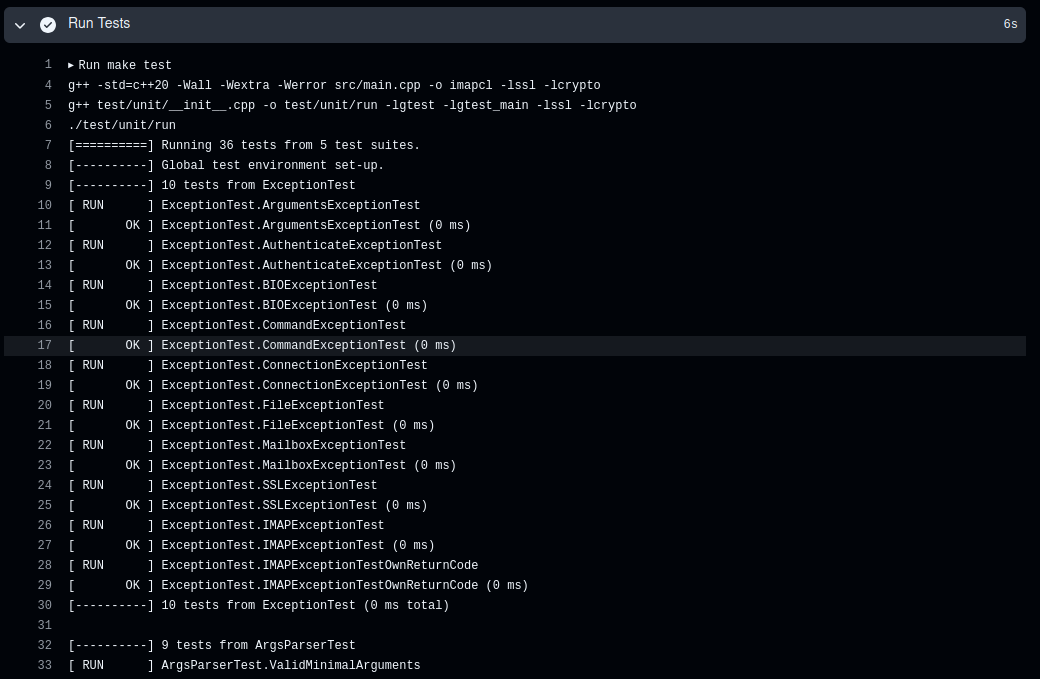
\includegraphics[width=0.9\linewidth]{res/test_unit.png}
		\caption{Zobrazenie jednotkových testov na GitHube.}
		\label{figure:testunit}
	\end{figure}

	\subsection{Systémové testy}
	Systémové testy prebehli manuálnym overovaním pripojenia k serveru. Pomocou nástroja Wireshark bola analyzovaná sieťová komunikácia, vrátane TLS paketov. Na priloženom obrázku nižšie je zobrazený príklad zachyteného TLS paketu, ktorý zobrazuje zabezpečené spojenie s poštovým serverom.\newline
	Ďaľším príkladom na inom obrázku je spustenie programu a overenie stiahnutia dvoch správ.\newline
	Pre účely detailnejšieho debugovania je k dispozícii debug verzia programu, ktorú je možné vygenerovať pomocou príkazu \texttt{make debug}. Výsledný spúšťateľný súbor \texttt{imapcl\_debug} poskytuje podrobné informácie o priebehu programu, ako je tiež možné vidieť na ostatnom obrázku.

	\label{subsection:testwireshark}
	\begin{figure}[!ht]
		\centering
		\vspace{1cm}
		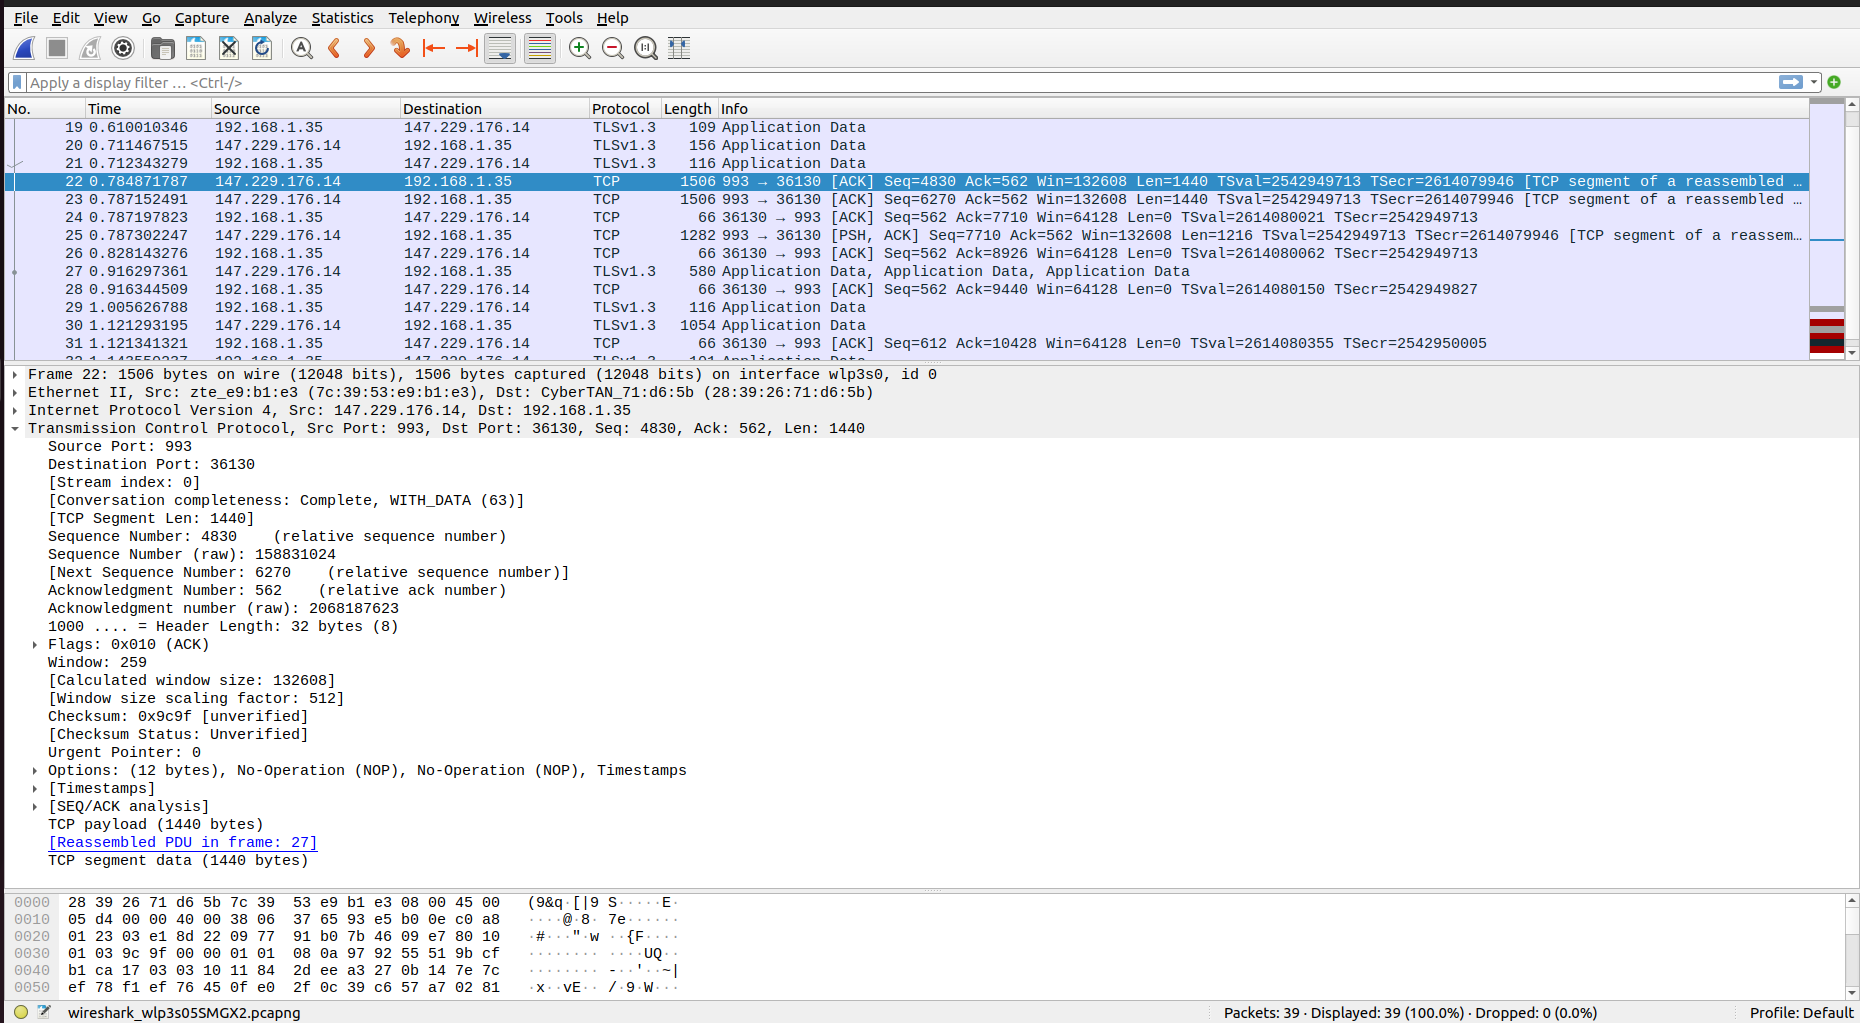
\includegraphics[width=0.9\linewidth]{res/test_wireshark.png}
		\caption{Príklad nezabezpečenej IMAP komunikácie v programe Wireshark.}
		\label{figure:testwireshark}
	\end{figure}
	\label{subsection:testbasic}
	\begin{figure}[!ht]
		\centering
		\vspace{1cm}
		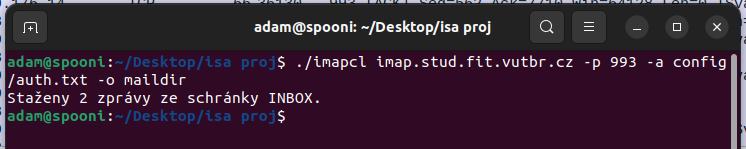
\includegraphics[width=0.9\linewidth]{res/test_basic.png}
		\caption{Obyčajné spustenie programu.}
		\label{figure:testbasic}
	\end{figure}
	\label{subsection:testdebug}
	\begin{figure}[!ht]
		\centering
		\vspace{1cm}
		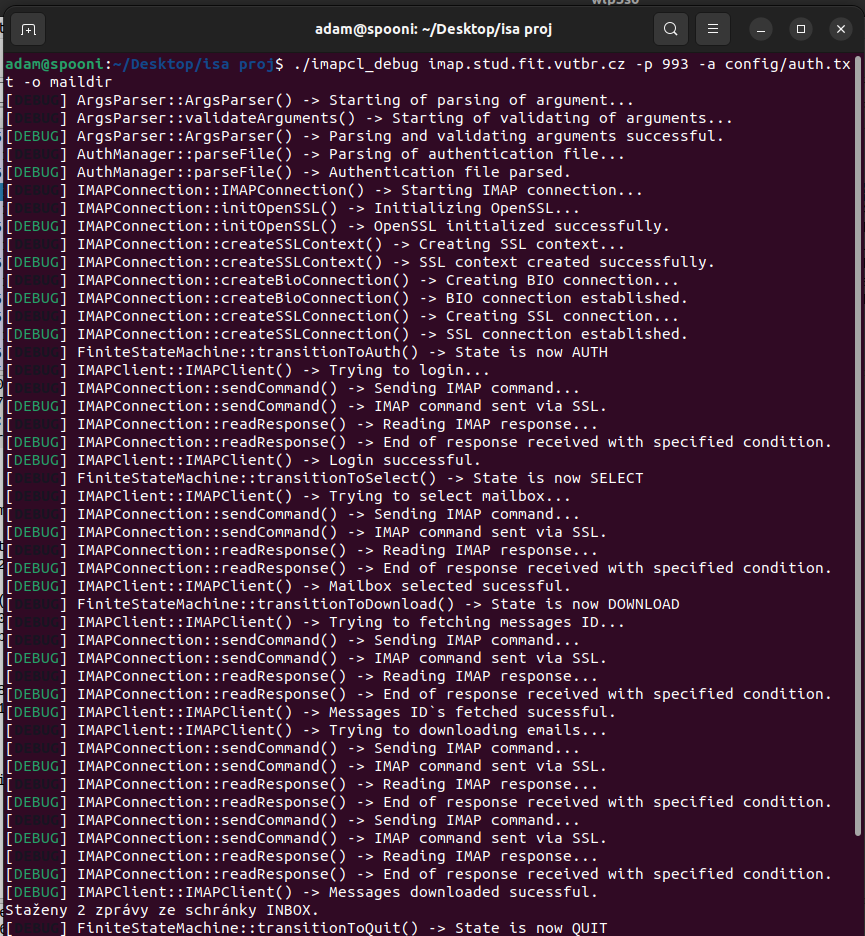
\includegraphics[width=0.9\linewidth]{res/test_debug.png}
		\caption{Spustenie debugovacích informácií.}
		\label{figure:testdebug}
	\end{figure}

	\subsection{Testy pamäte}
	Sú vykonávané vďaka nástroju Valgrind a GitHub workflow-u. Ten pri každom nahratí novej verzie vykoná príkaz \texttt{make valgrind}, ktorý spustí Valgrind analýzu. Následne prebehne kontrola, ktorá zaistí, či výsledný súbor obsahuje reťazec \texttt{ERROR SUMMARY: 0 errors from 0 contexts}, teda či je všetka práca s pamäťou správna. Výstup valgrind testov je možné vidieť na obrázku nižšie.
	\label{subsection:testvalgrind}
	\begin{figure}[!ht]
		\centering
		\vspace{1cm}
		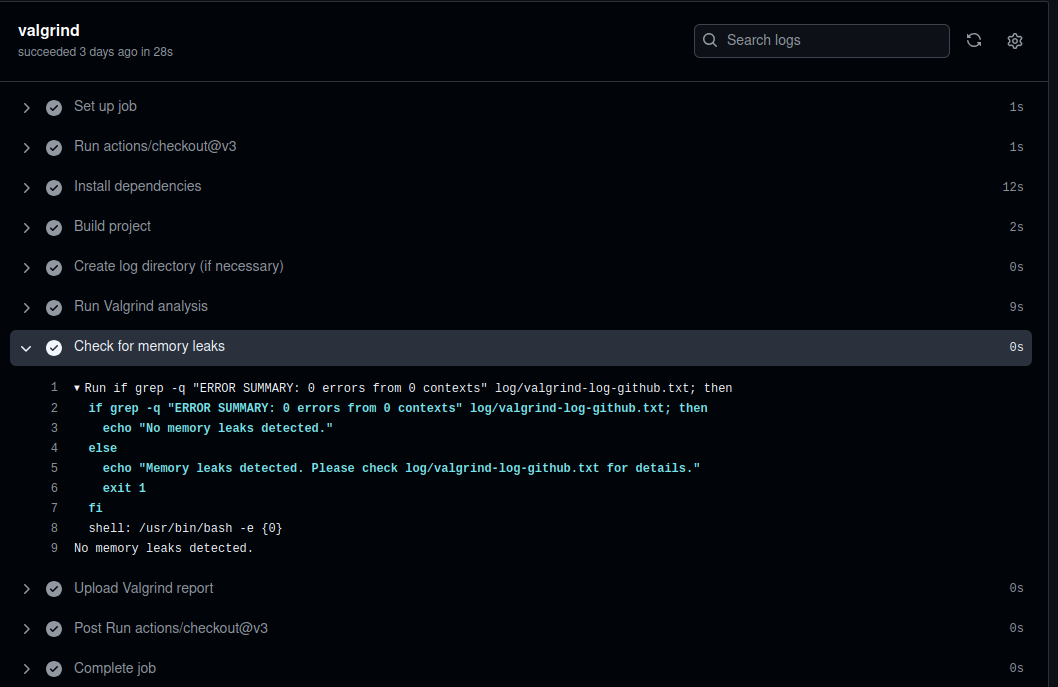
\includegraphics[width=0.9\linewidth]{res/test_valgrind.png}
		\caption{Zobrazenie výstupu valgrind testu na GitHube.}
		\label{figure:testvalgrind}
	\end{figure}


	%%%%% Literatúra %%%%%
    \clearpage
	\section{Literatúra}
	\bibliographystyle{bib/czechiso}
    \renewcommand{\refname}{}
	\bibliography{bib/manual}

	%%%%% Prílohy %%%%%
    \clearpage
	\appendix
	\section{Prílohy}
    \subsection{Diagram prípadov použitia}
	\label{subsection:usecase}
	\begin{figure}[!ht]
		\centering
		\vspace{1cm}
		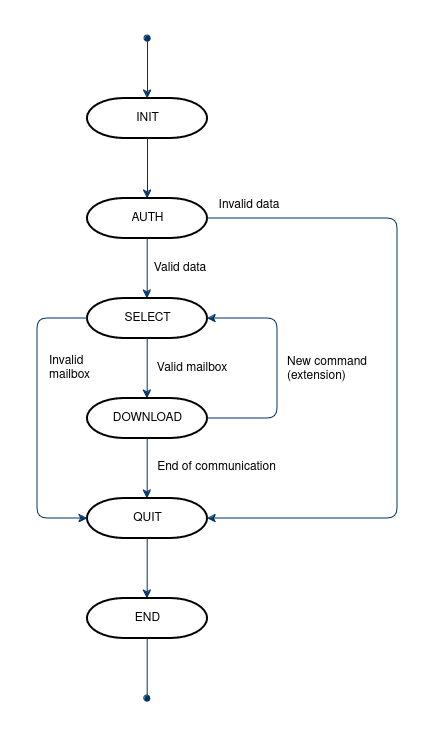
\includegraphics[width=0.5\linewidth]{res/diagram_usecase.png}
		\caption{Diagram prípadov použitia}
		\label{figure:usecase}
	\end{figure}

	\clearpage
	\subsection{Diagram tried}
	\label{subsection:class}
	\begin{figure}[!ht]
		\centering
		\vspace{1cm}
		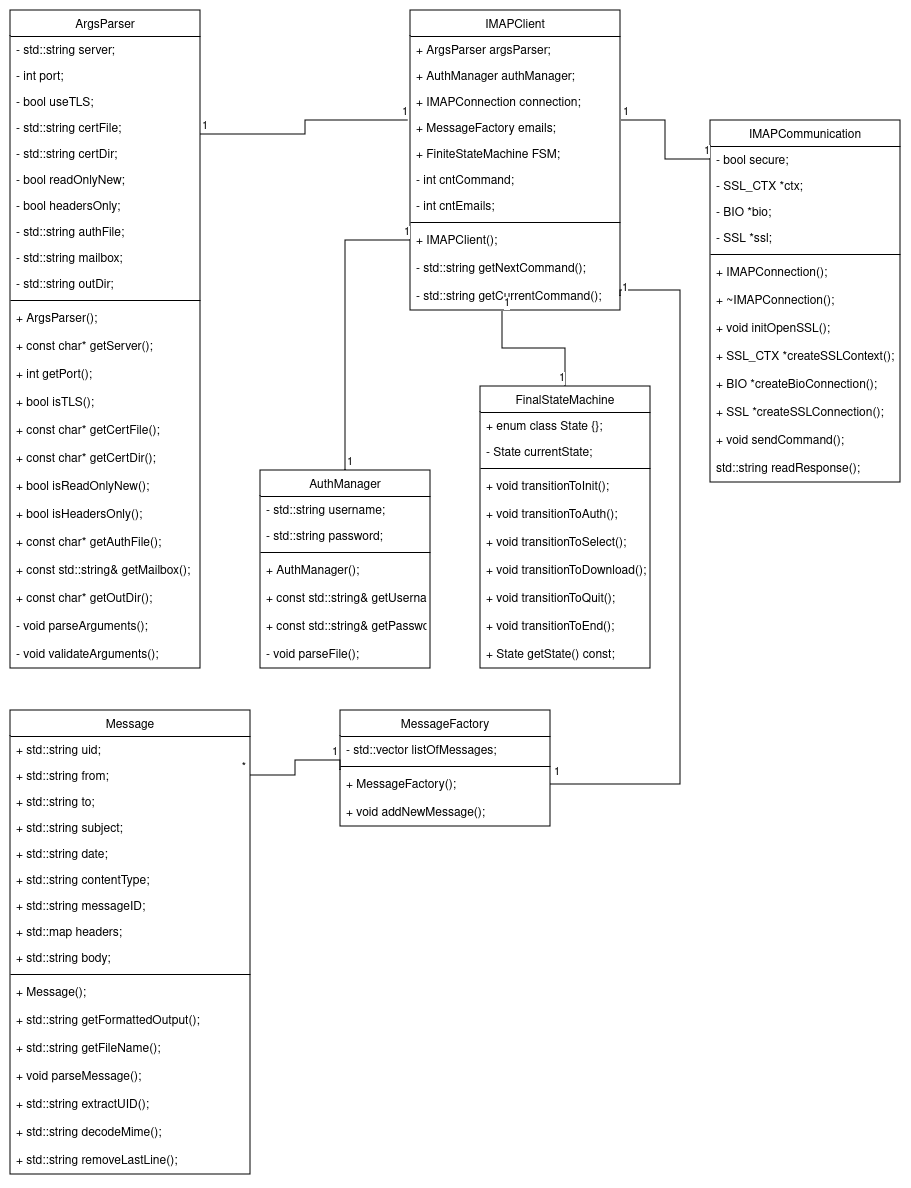
\includegraphics[width=0.9\linewidth]{res/diagram_class.png}
		\caption{Diagram tried}
		\label{figure:class}
	\end{figure}

	\clearpage
	\subsection{Diagram sekvencie}
	\label{subsection:sequence}
	\begin{figure}[!ht]
		\centering
		\vspace{1cm}
		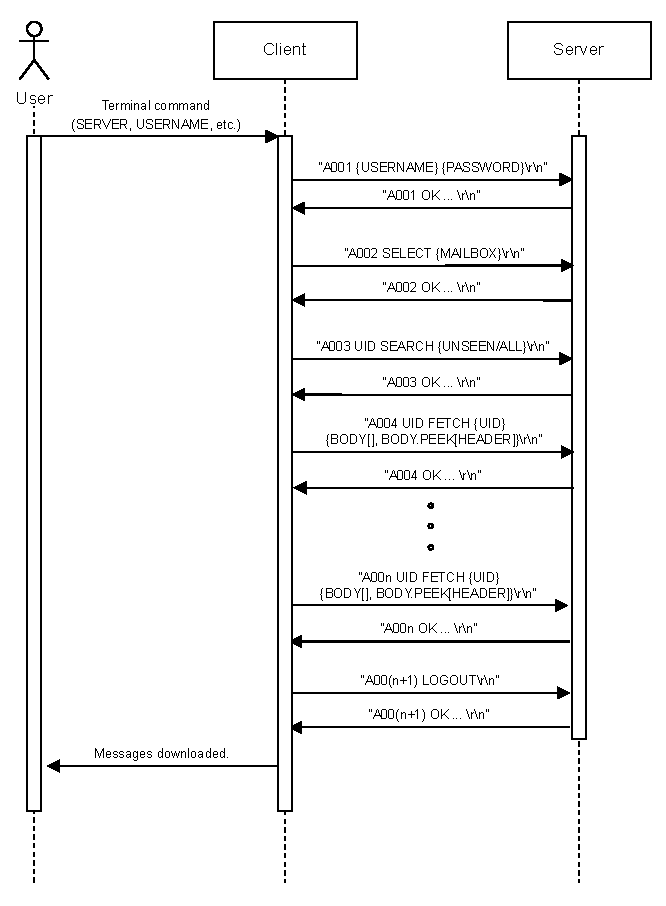
\includegraphics[width=0.9\linewidth]{res/diagram_sequence.pdf}
		\caption{Diagram sekvencie: jednoduchá komunikácia používateľa so serverom pomocou klienta.}
		\label{figure:sequence}
	\end{figure}

\end{document}